\documentclass[../main.tex]{subfiles}
\begin{document}
\captionsetup{font=small}
\appendix
\pagenumbering{Roman} 

%\addcontentsline{toc}{section}{Appendix A: Full List of Used Instruments}
\section{Full List of Used Instruments}
\label{appendix:instruments}
\noindent 3 scintillating planes, each one containing:
\begin{itemize}
    \item 2 Plastic scintillator planes
    \item 2 Hamamatsu H316504 photomultipliers
    \item 1 High-Voltage input connector
    \item 2 LEMO output connectors
\end{itemize}
The rack contains:
\begin{itemize}
    \item CAEN N840 8-Channel Leading Edge Discriminator (LED)
    \item CAEN N455 Quad Coincidence Logic Unit
    \item CAEN N405 3 Fold Logic Unit
    \item CAEN N108A Dual Delay% ritardare p1 e p2 al trigger
    \item CAEN N1145 Quad Scaler and Preset Counter Timer
    \item CAEN N93B Dual Timer
\end{itemize}
Miscellaneous:
\begin{itemize}
    \item LEMO coaxial cables
    \item RS PRO IDS1104B Oscilloscope (previously Tektronix TDS 2024 Oscilloscope)
    \item Digilent Cmod Spartan-7 FPGA
    \item Two 4 cm concrete blocks
    \item Two 0.5 cm iron plates
\end{itemize}
Software:
\begin{itemize}
    \item GEneral COntrol (GECO) software 2020
    \item Python Version 3.10.6
    \item ROOT CERN Version 6.26/06
    \item \LaTeX \phantom{ } pdfTeX, Version 3.141592653-2.6-1.40.24 (\TeX \phantom{}  Live 2022)
\end{itemize}

%\addcontentsline{toc}{section}{Appendix B: Data and Tables}
\clearpage
\section{Data and Tables}
%\addcontentsline{toc}{subsection}{Setup Measurements}
\subsection{Setup Measurements}
\noindent Reference planes calibration counts taken from the shared folder.
\FloatBarrier

    %HV 1B, HV 2B, HV 3B, THR 1B, THR 2B, THR 3B
    \FloatBarrier
    \begin{table}[h!]
        \centering
        \caption{Measured counts for varying voltage for PMTs 11 and 12 at \SI{20}{\milli \volt} threshold. Reference scintillators are 01 and 02, set at \SI{1000}{\volt} tension, \SI{20}{\milli \volt} threshold. Each setting has been taking data for \SI{100}{\second}. Measures were performed by group 1B. The highlighted line probably contains a transcription error since coincidence counts are not expected to exceed single counts.}%The highlighted line probably contains a transcription error since coincidence counts are not expected to exceed single counts.
         \label{tab:HV1B}
            \begin{NiceTabular}{|c|cc|cc|}[colortbl-like]
            \hline
            HV (V) & PMT11 singles & PMT12 singles & PMT11 coinc & PMT12 coinc \\ \hline
           \rowcolor{red!15} \phantom{0}700    & \phantom{000}10            & \phantom{000}11            & \phantom{00}11          & \phantom{00}16          \\
            \phantom{0}750    & \phantom{000}79            & \phantom{00}119           & \phantom{00}55          & \phantom{00}89          \\
            \phantom{0}800    & \phantom{00}321           & \phantom{00}471           & \phantom{0}273         & \phantom{0}376         \\
            \phantom{0}850    & \phantom{0}1108          & \phantom{0}1690          & \phantom{0}795         & 1132        \\
            \phantom{0}900    & \phantom{0}2508          & \phantom{0}3459          & 1368        & 1521        \\
            \phantom{0}950    & \phantom{0}4378          & \phantom{0}5919          & 1539        & 1597        \\
            1000   & \phantom{0}6848          & \phantom{0}9126          & 1458        & 1496        \\
            1050   & 11592         & 14096         & 1623        & 1668        \\
            1100   & 22598         & 22078         & 1657        & 1758        \\ \hline
        \end{NiceTabular}
    \end{table}
    
    \begin{table}[b!]
        \centering
        \caption{Measured counts for varying threshold for PMTs 11 and 12 at \SI{1000}{\volt} tension. Reference scintillators are 01 and 02, set at \SI{1000}{\volt} tension, \SI{5}{\milli \volt} threshold. Each setting has been taking data for \SI{100}{\second}. Measures were performed by group 1B.}
        \label{tab:threshold1B}
            \begin{tabular}{|c|cc|cc|}
            \hline
            Thr (mV) & PMT11 singles & PMT12 singles & PMT11 coinc & PMT12 coinc \\ \hline
            \phantom{0}5        & 48297         & 38194         & 2660        & 3075        \\
            \phantom{0}7        & 28743         & 24974         & 2383        & 2700        \\
            10       & 15321         & 16293         & 2124        & 2341        \\
            15       & \phantom{0}9243          & 11498         & 1887        & 2035        \\
            20       & \phantom{0}6802          & \phantom{0}7018          & 1766        & 1891        \\
            25       & \phantom{0}5335          & \phantom{0}8899          & 1605        & 1712        \\
            30       & \phantom{0}4374          & \phantom{0}5895          & 1581        & 1666        \\
            32       & \phantom{0}5088          & \phantom{0}5531          & 1501        & 1596        \\
            35       & \phantom{0}3592          & \phantom{0}4929          & 1434        & 1563        \\
            40       & \phantom{0}3102          & \phantom{0}4386          & 1447        & 1623        \\
            41       & \phantom{0}3035          & \phantom{0}4281          & 1455        & 1598        \\
            45       & \phantom{0}2583          & \phantom{0}3769          & 1343        & 1542        \\
            50       & \phantom{0}2190          & \phantom{0}3192          & 1244        & 1512        \\
            60       & \phantom{0}1579          & \phantom{0}2403          & 1040        & 1382        \\
            70       & \phantom{0}1166          & \phantom{0}1955          & \phantom{0}848         & 1285        \\ \hline
            \end{tabular}
        \end{table}
        \FloatBarrier
%2%%%%%%%%%%%%%%%%%%%%%%%%%%%%%%%%%%%%%%%%%%%%%%%%%%%%%%%
    \begin{table}[t!]
    \centering
    \caption{Measured counts for varying voltage for PMTs 01 and 02 at \SI{35}{\milli \volt} threshold. Reference scintillators are 11 and 12, set at \SI{1000}{\volt} tension, \SI{35}{\milli \volt} threshold. Each setting has been taking data for \SI{100}{\second}. Measures were performed by group 2B.}
    \label{tab:HV2B}
    %\resizebox{\textwidth}{!}{%
    \begin{tabular}{|c|cc|cc|}
    \hline
    HV (V)  & PMT01 singles & PMT02 singles & PMT01 coinc & PMT02 coinc \\ \hline
    \phantom{0}700  & \phantom{0000}2             & \phantom{0000}8             & \phantom{000}1           & \phantom{000}5           \\
    \phantom{0}800  & \phantom{000}72            & \phantom{00}342           & \phantom{00}58          & \phantom{0}272         \\
    \phantom{0}850  & \phantom{00}346           & \phantom{0}1178          & \phantom{0}293         & \phantom{0}876         \\
    \phantom{0}900  & \phantom{0}1211          & \phantom{0}2776          & \phantom{0}894         & 1332        \\
    \phantom{0}950  & \phantom{0}2637          & \phantom{0}5218          & 1320        & 1404        \\
    1000 & \phantom{0}4775          & \phantom{0}8193          & 1415        & 1450        \\
    1050 & \phantom{0}7824          & 13318         & 1454        & 1483        \\
    1100 & 12281         & 24090         & 1431        & 1487        \\ \hline
    \end{tabular}%
    %}
    \end{table}
    
    \begin{table}[b!]
            \centering
            \caption{Measured counts for varying threshold for PMTs 01 and 02 at \SI{1000}{\volt} tension. Reference scintillators are 11 and 12, set at \SI{1000}{\volt} tension, \SI{5}{\milli \volt} threshold. Each setting has been taking data for \SI{100}{\second}. Measures were performed by group 2B.}
            \label{tab:threshold2B}
                \begin{tabular}{|c|cc|cc|}
                    \hline
                    Thr (mV) & PMT01 singles & PMT02 singles & PMT01 coinc & PMT02 coinc \\ \hline
                    \phantom{00}5        & 51654         & 82069         & 3043        & 3338        \\
                    \phantom{0}15       & 12065         & 25039         & 2112        & 2543        \\
                    \phantom{0}25       & \phantom{0}6991          & 12054         & 1741        & 1955        \\
                    \phantom{0}35       & \phantom{0}4801          & \phantom{0}8554          & 1626        & 1789        \\
                    \phantom{0}45       & \phantom{0}3389          & \phantom{0}6417          & 1555        & 1722        \\
                    \phantom{0}50       & \phantom{0}2865          & \phantom{0}5495          & 1489        & 1683        \\
                    \phantom{0}60       & \phantom{0}2081          & \phantom{0}4285          & 1323        & 1553        \\
                    \phantom{0}75       & \phantom{0}1425          & \phantom{0}3250          & 1067        & 1487        \\
                    \phantom{0}85       & \phantom{0}1070          & \phantom{0}2509          & \phantom{0}840         & 1387        \\
                    100      & \phantom{00}593           & \phantom{0}1730          & \phantom{0}492         & 1131        \\
                    150      & \phantom{000}79            & \phantom{00}202           & \phantom{00}64          & \phantom{0}137         \\ \hline
                \end{tabular}
        \end{table}
        \FloatBarrier
        \begin{table}[t!]
            \centering
            \caption{Measured counts for varying voltage for PMTs 03 and 04 at \SI{40}{\milli \volt} threshold. Reference scintillators are 11 and 12, set at \SI{1000}{\volt} tension, \SI{40}{\milli \volt} threshold. Each setting has been taking data for \SI{100}{\second}. Measures were performed by group 3B.}
            \label{tab:HV3B}
                \begin{tabular}{|c|cc|cc|}
                    \hline
                    HV (V) & PMT03 singles & PMT04 singles & PMT03 coinc & PMT04 coinc \\ \hline
                    \phantom{0}800 & \phantom{000}77 & \phantom{000}45 & \phantom{00}52 & \phantom{00}22 \\
                    \phantom{0}850 & \phantom{00}338 & \phantom{00}199 & \phantom{0}226 & \phantom{0}114 \\
                    \phantom{0}900 & \phantom{0}1241 & \phantom{00}736 & \phantom{0}777 & \phantom{0}459 \\
                    \phantom{0}950 & \phantom{0}2606 & \phantom{0}1767 & 1108           & \phantom{0}958 \\
                    1000           & \phantom{0}5142 & \phantom{0}3570 & 1163           & 1128        \\
                    1050           & \phantom{0}8660 & \phantom{0}6076 & 1241           & 1236        \\
                    1100           & 13227           & 10051           & 1250           & 1241        \\
                    1150           & 26367           & 15546           & 1137           & 1119        \\ \hline
                \end{tabular}
        \end{table}
\begin{table}[b!]
    \centering
    \caption{Measured counts for varying threshold for PMTs 03 and 04 at \SI{1000}{\volt}  tension. Reference scintillators are 11 and 12, set at \SI{1000}{\volt} tension, \SI{2}{\milli \volt} threshold. Each setting has been taking data for \SI{100}{\second}. Measures were performed by group 3B.}
            \label{tab:threshold3B}
        \begin{tabular}{|c|cc|cc|}
        \hline
        Threshold (mV) & PMT03 singles & PMT04 singles & PMT03 coinc & PMT04 coinc \\ \hline
        \phantom{00}2 & 107042           & 91962           & 4307        & 4683        \\
        \phantom{00}5 & \phantom{0}65890 & 62027           & 3327        & 3635        \\
        \phantom{0}10 & \phantom{0}27114 & 23604           & 2379        & 2408        \\
        \phantom{0}15 & \phantom{0}14997 & 12896           & 1923        & 1848        \\
        \phantom{0}20 & \phantom{0}10787 & \phantom{0}9139 & 1684        & 1606        \\
        \phantom{0}25 & \phantom{00}8433 & \phantom{0}7021 & 1599        & 1521        \\
        \phantom{0}30 & \phantom{00}6901 & \phantom{0}5362 & 1525        & 1466        \\
        \phantom{0}35 & \phantom{00}5721 & \phantom{0}4459 & 1487        & 1421        \\
        \phantom{0}40 & \phantom{00}4842 & \phantom{0}3682 & 1417        & 1357        \\
        \phantom{0}45 & \phantom{00}4090 & \phantom{0}2887 & 1317        & 1237        \\
        \phantom{0}50 & \phantom{00}3555 & \phantom{0}2619 & 1318        & 1234        \\
        \phantom{0}60 & \phantom{00}2557 & \phantom{0}1794 & 1230        & 1056        \\
        \phantom{0}70 & \phantom{00}1939 & \phantom{0}1339 & 1103        & \phantom{0}836 \\
        \phantom{0}80 & \phantom{00}1440 & \phantom{00}955 & \phantom{0}940 & \phantom{0}640 \\
        \phantom{0}90 & \phantom{00}1063 & \phantom{00}623 & \phantom{0}689 & \phantom{0}410 \\
        120           & \phantom{000}228 & \phantom{00}174 & \phantom{0}152 & \phantom{0}101 \\
        160           & \phantom{0000}20 & \phantom{000}41 & \phantom{000}5 & \phantom{00}10 \\
        200           & \phantom{00000}0 & \phantom{000}26 & \phantom{000}0 & \phantom{000}0 \\ \hline
        \end{tabular}
\end{table}
        

        \FloatBarrier
%%%%%%%%%%%%%%%%%%%%%%%%%%%%%%%%%%%%%%%%%%%%%%%%%%%%%%%%%%%%%%%%%%%%%%%%%%%%55
        \begin{table}[ht]
            \centering
            \caption{Measured plane efficiencies}
            \label{tab:efficiencies}
                \resizebox{\textwidth}{!}{%
                \begin{tabular}{|c|c|c|c|}
                \hline
                \multicolumn{1}{|l|}{Plane} &
                  \multicolumn{1}{l|}{Triple coincidence counts (Trip)} &
                  \multicolumn{1}{l|}{Reference Counts (Ref)} &
                  \multicolumn{1}{l|}{Efficiency (Trip/Ref)} \\ \hline
                P1 & 1298 & 1337 & 97\% \\
                P2 & 1225 & 1274 & 96\% \\
                P3 & 1359 & 1406 & 97\% \\ \hline
                \end{tabular}
                }
        \end{table}
    \FloatBarrier
\subsection{Data Taking}
    \begin{figure}[htb!]
        \centering
        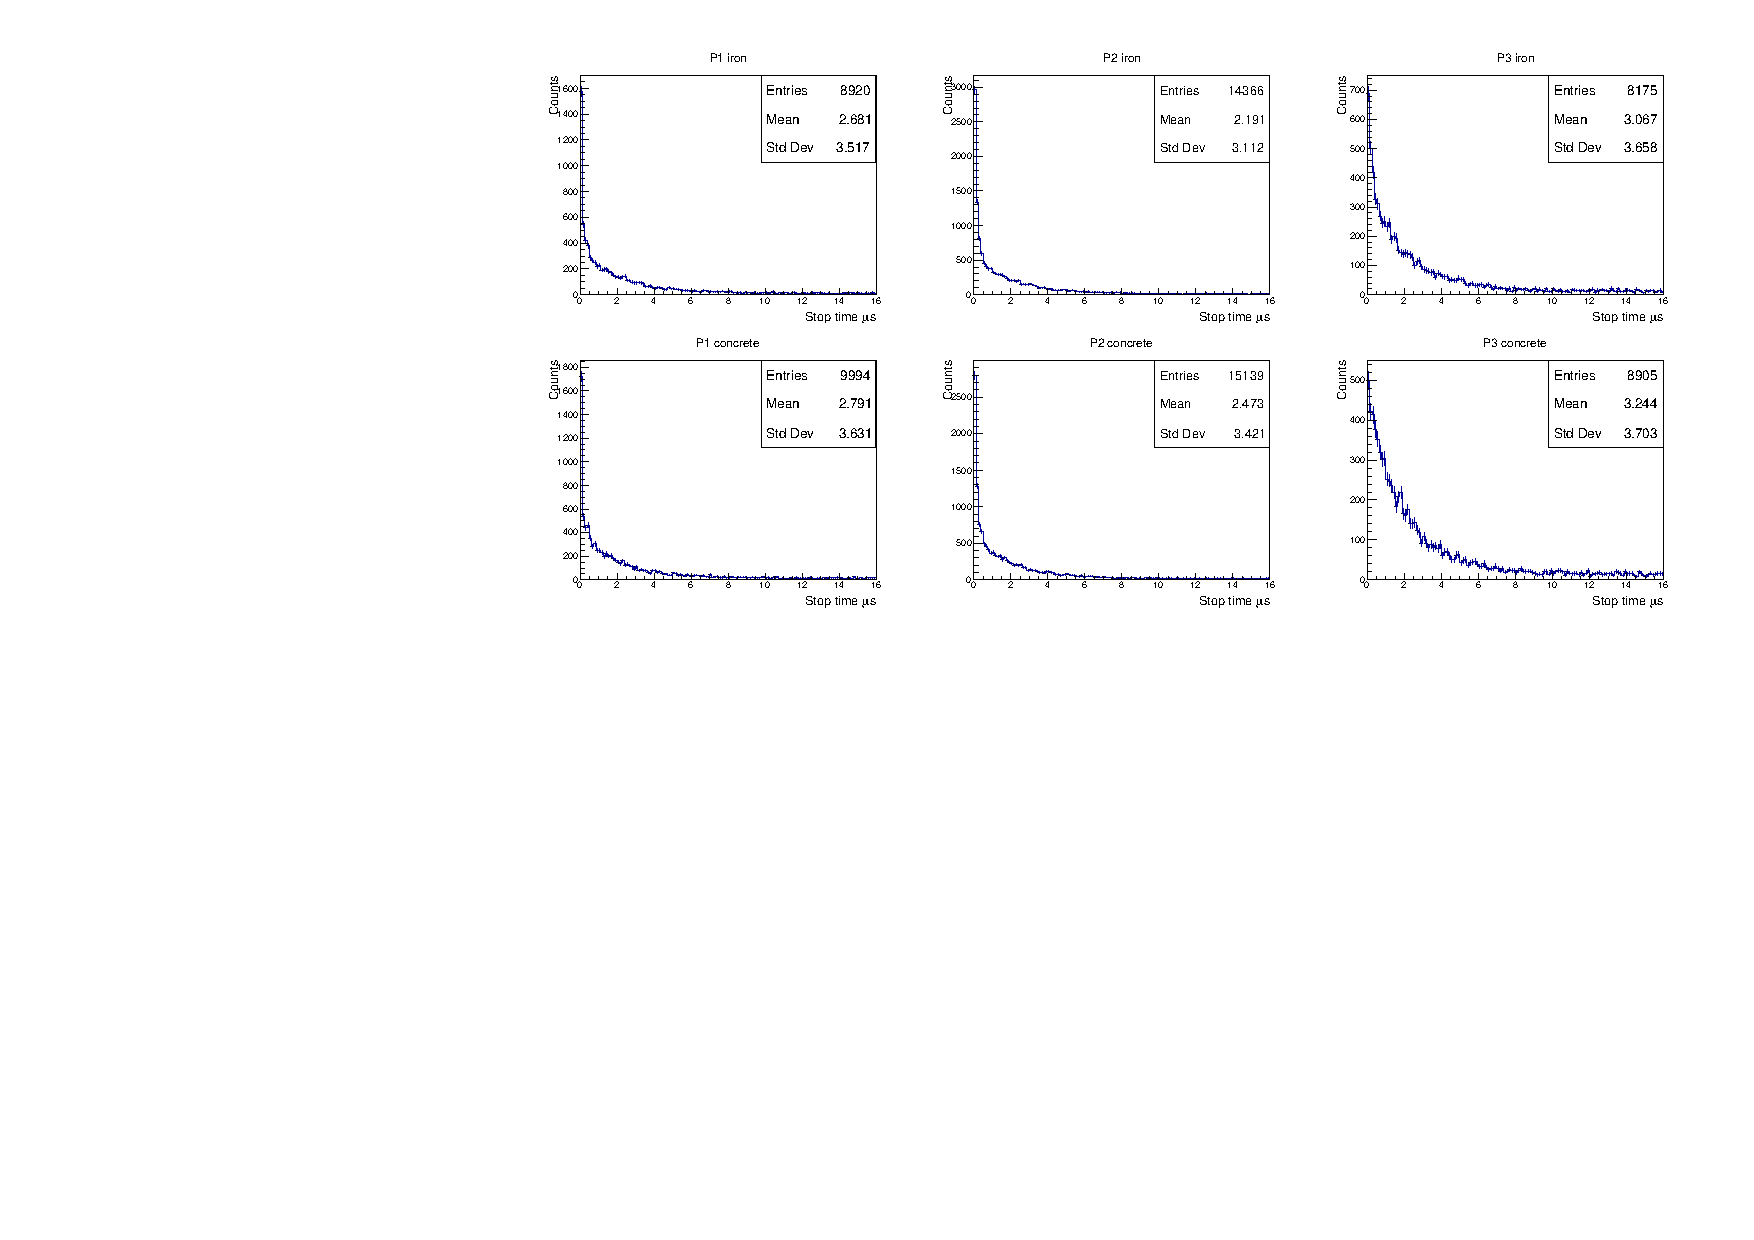
\includegraphics[width=\linewidth]{images/histograms.pdf}
        \caption{Raw histograms of the acquired data. As stated in Section \ref{sec:res} a strong double spike, probably due to PMT afterpulses, is visible in the first bins of the histograms of P1 and P2 for both absorbers.}
        \label{fig:rawHisto}
    \end{figure}
\FloatBarrier

     \begin{figure}[htb!]
         \centering
         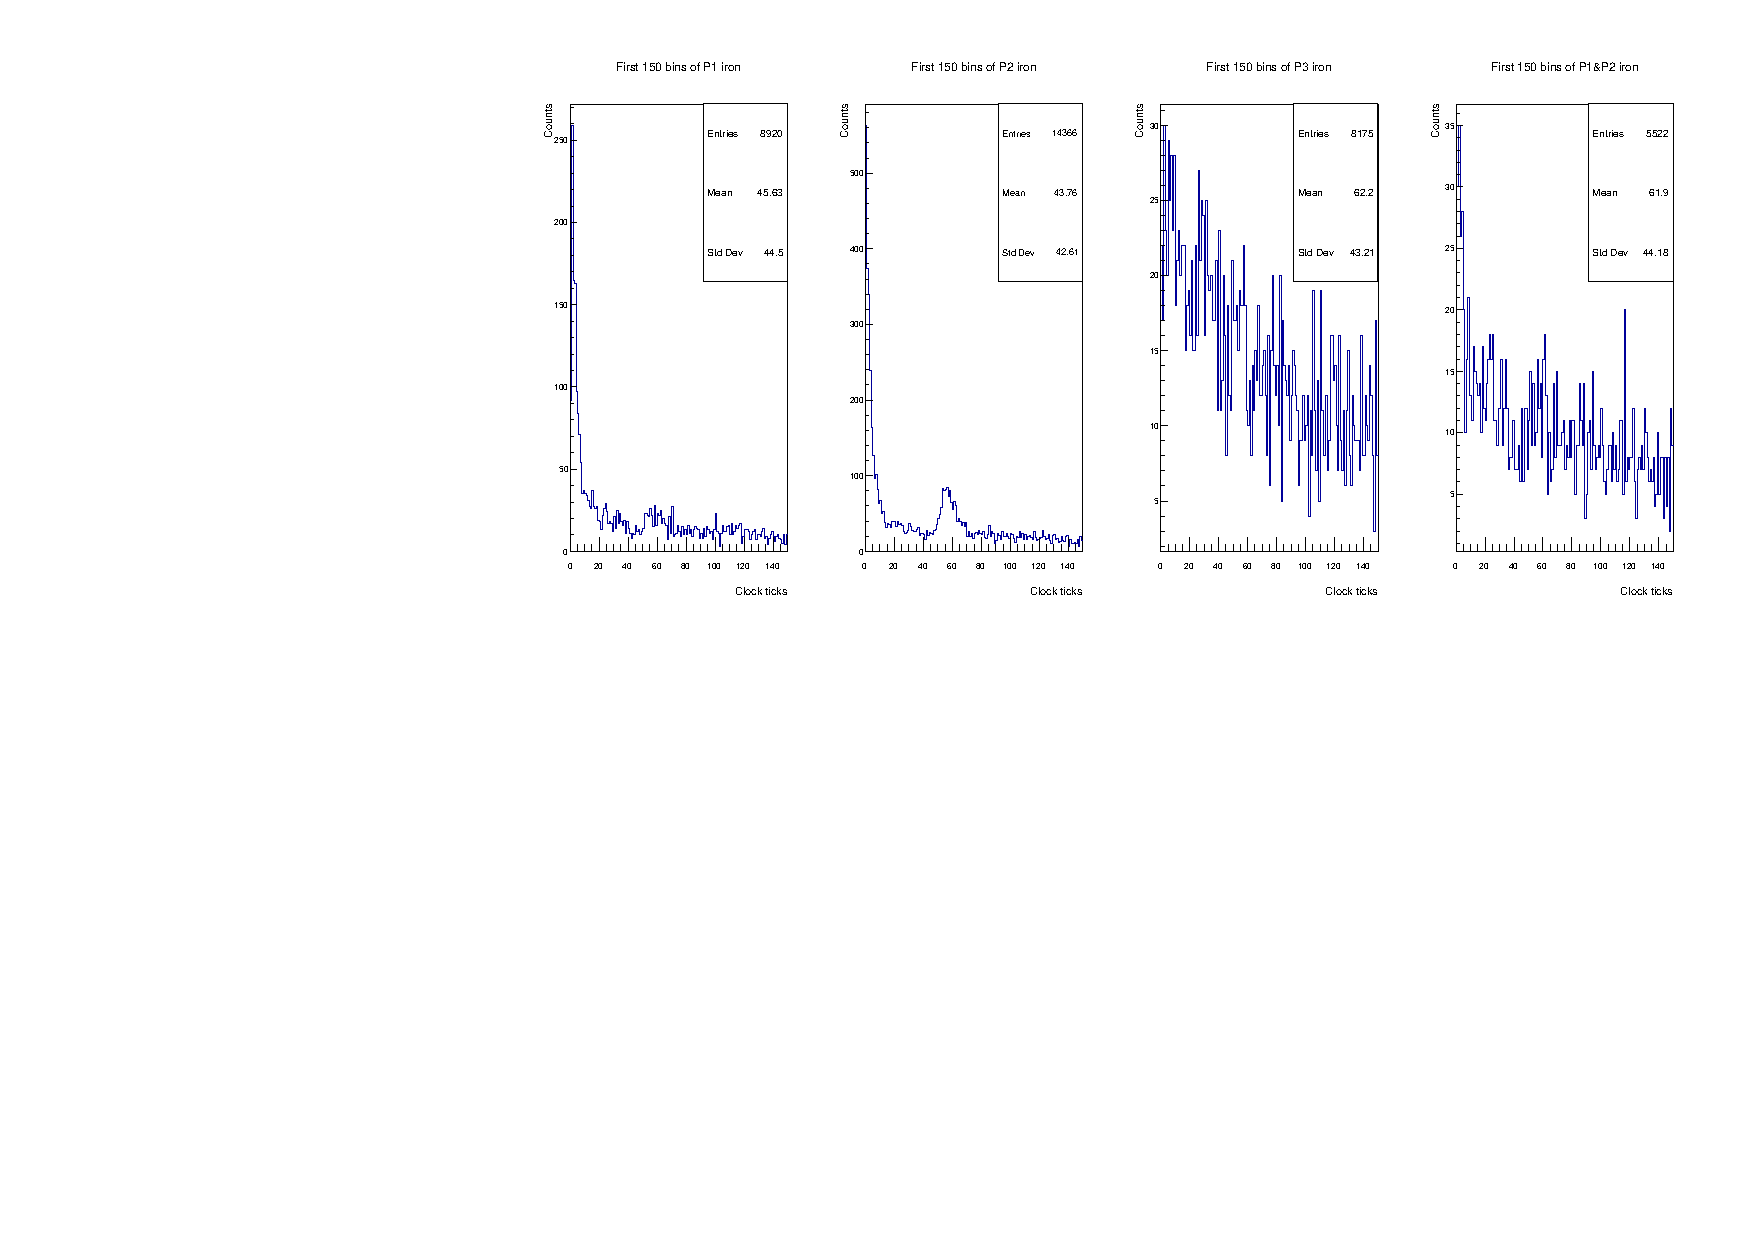
\includegraphics[width=\linewidth]{images/first_150_iron_bins.pdf}
         \caption{Zoom in on the first 150 clock cycles stops for iron absorber. Around 60 clock cycles (\textnormal{240\,ns}) a spike compatible with a long-timescale afterpulse is visible on P2. The big peak before 10  clock cycles (\textnormal{40\,ns}) may be due to short-timescale  afterpulses or some other effects on the setup. In any case a partial suppression of these effects can be achieved via P1$\land$P2 event filtering.}
         \label{fig:150iron}
     \end{figure}

      \begin{figure}[htb!]
         \centering
         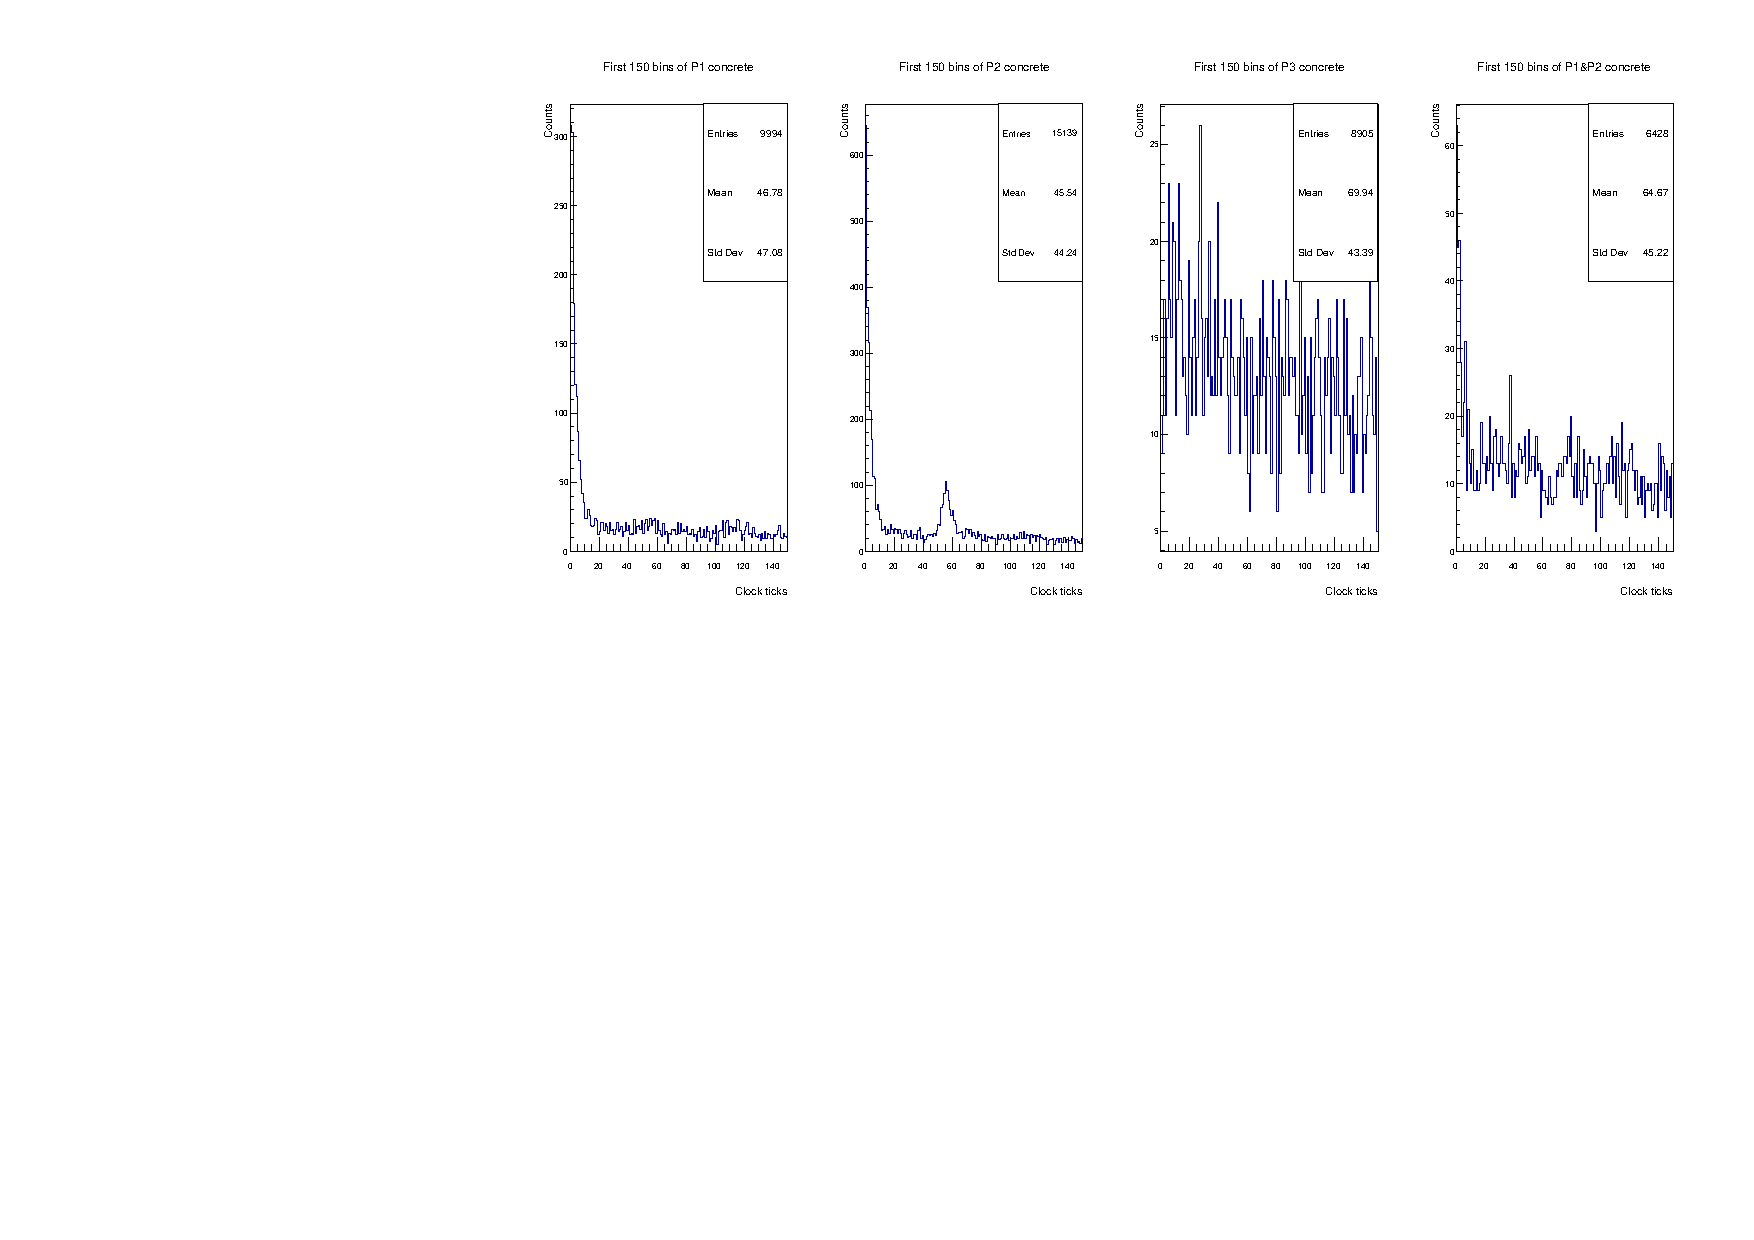
\includegraphics[width=\linewidth]{images/first_150_concrete_bins.pdf}
         \caption{Zoom in on the first 150 clock cycles stops for concrete absorber. Around 60 clock cycles (\textnormal{240\,ns}) a spike compatible with a long-timescale afterpulse is visible on P2. The big peak before 10  clock cycles (\textnormal{40\,ns}) may be due to short-timescale  afterpulses or some other effects on the setup. In any case a partial suppression of these effects can be achieved via P1$\land$P2 event filtering.}
         \label{fig:150concrete}
     \end{figure}

     \FloatBarrier

     \begin{figure}[htb!]
         \centering
         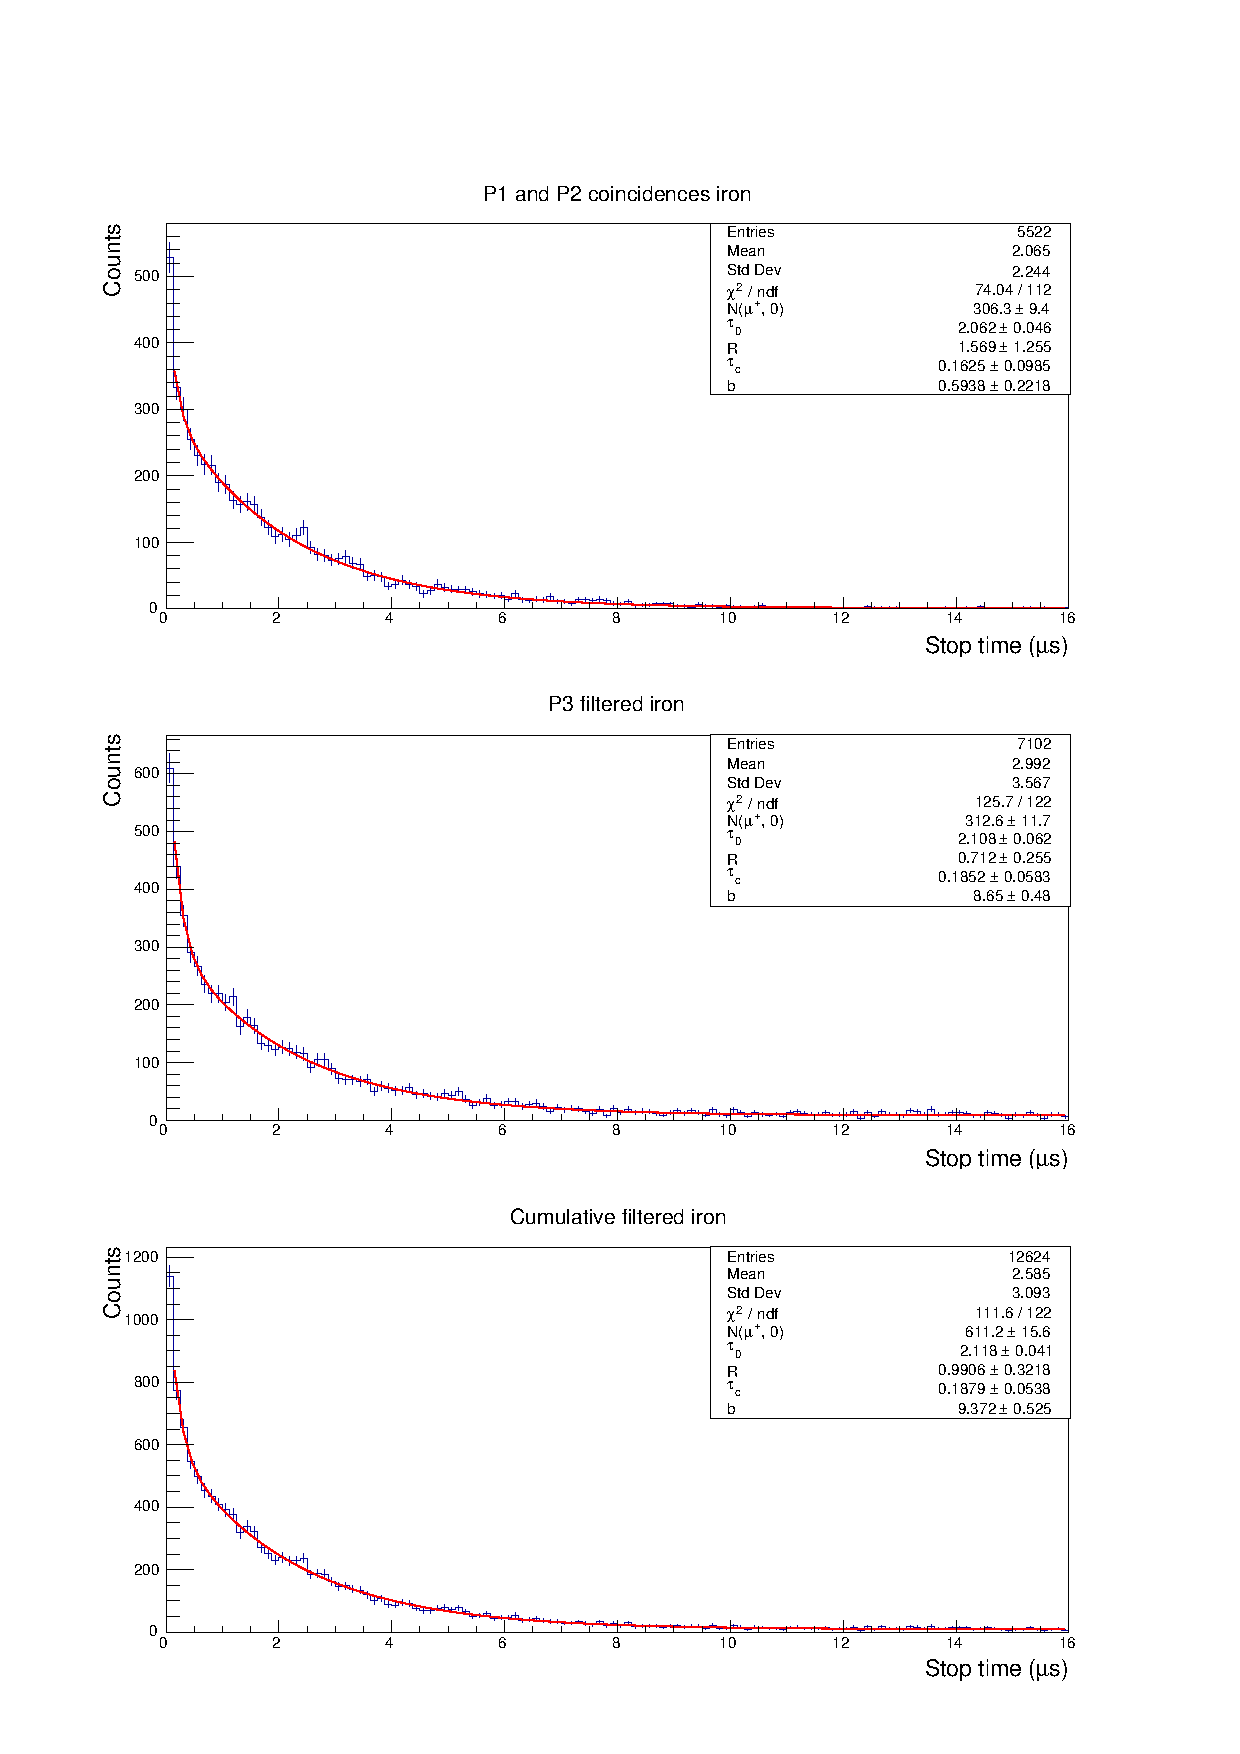
\includegraphics[width=0.9\linewidth]{images/1_over_r_iron_fit.pdf}
         \caption{Fit for iron absorber with filtered data leaving all parameters free.}
         \label{fig:allFreeIron}
     \end{figure}

    \begin{figure}[htb!]
         \centering
         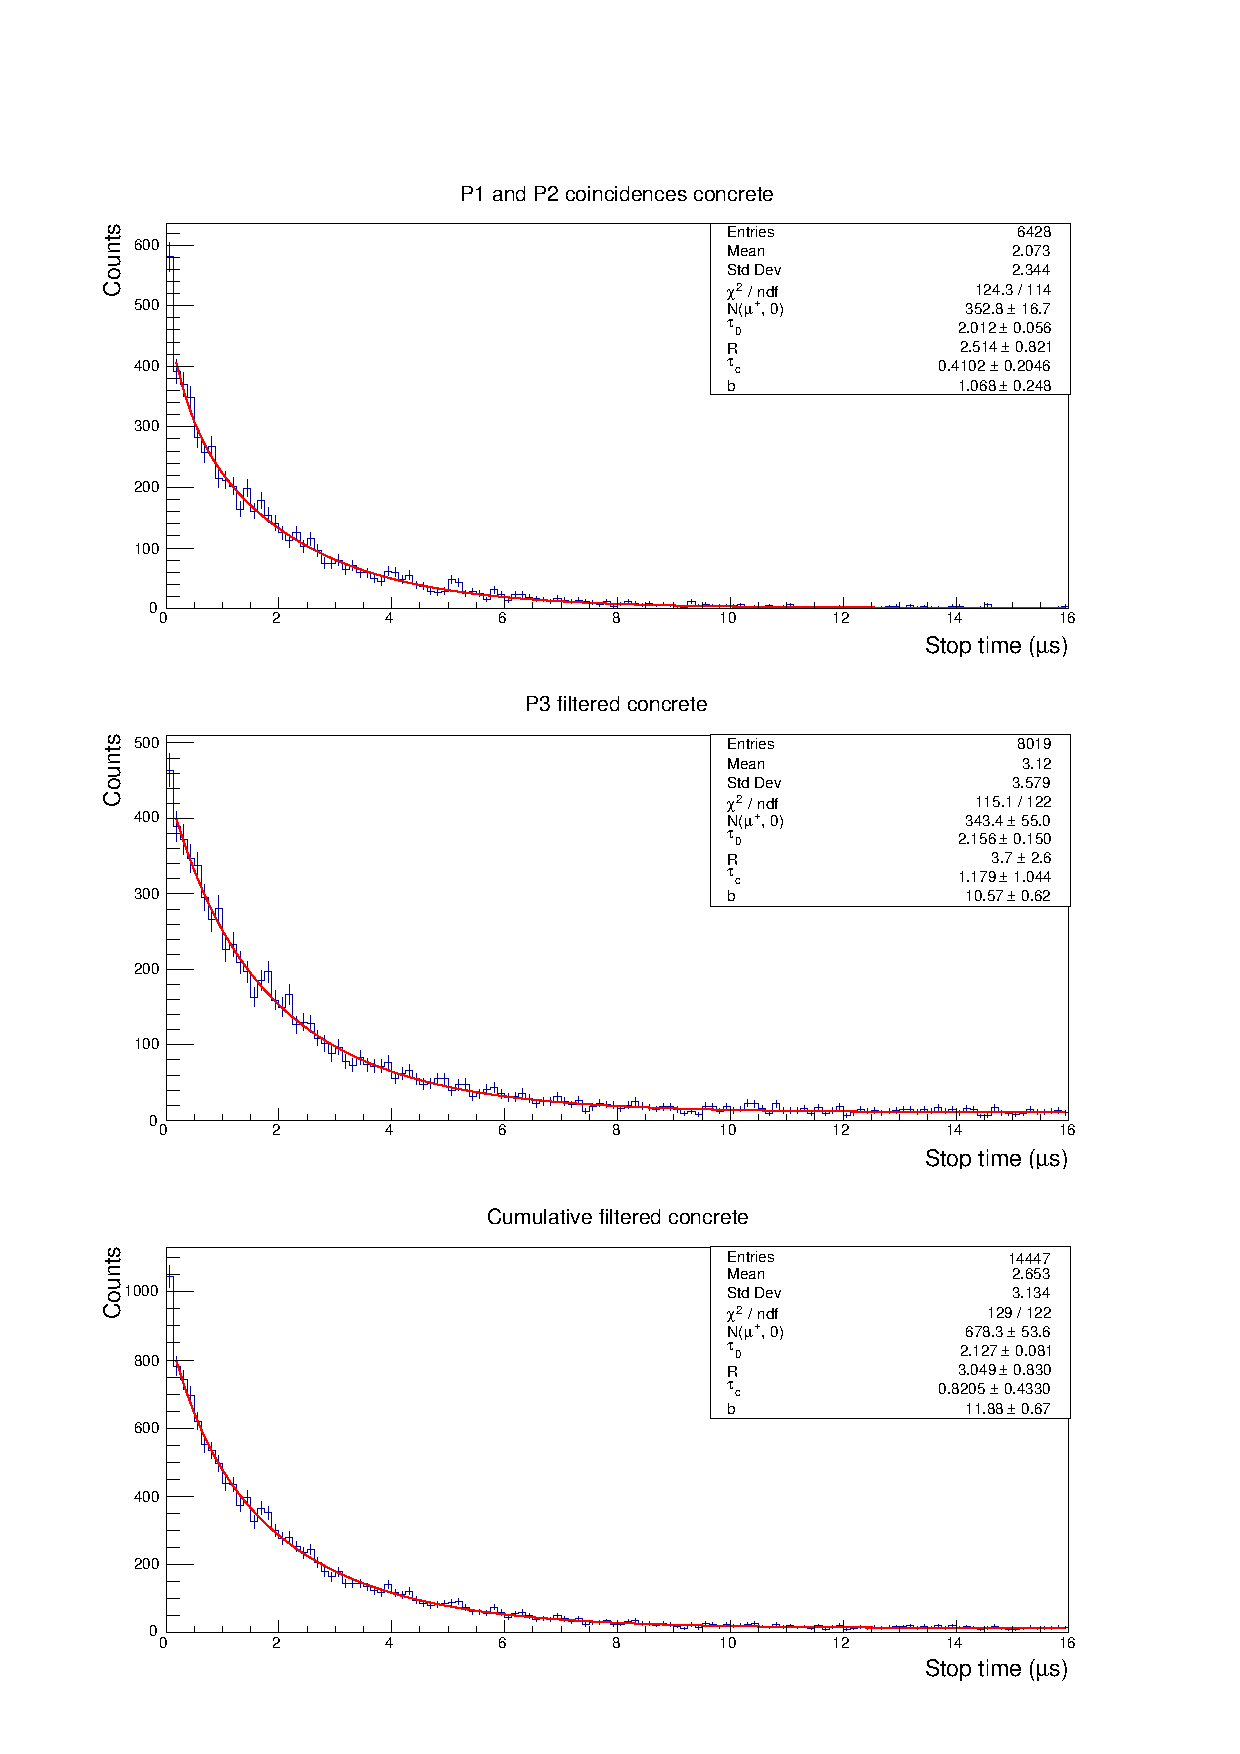
\includegraphics[width=0.9\linewidth]{images/1_over_r_concrete_fit.pdf}
         \caption{Fit for concrete absorber with filtered data leaving all parameters free.}
         \label{fig:allFreeConcrete}
     \end{figure}
\FloatBarrier
\section{Fit Choices}
During data analysis some decisions were taken regarding binning and fitting ranges. In order to avoid biasing the results doing selective handpicks, some limits were decided before fitting operations, limiting the prior-to-fit knowledge to only the pieces of information that could be gathered by looking at the workstation event display.\\

For what concerns binning, since the events featuring a stop were in the order of $10^4$ a good bin choice was thought to be around $10^2$. Moreover, the overflow stop time was \texttt{0xfff}, meaning $16^3=4096$ possible stop times. This led to opting for 128 bins, meaning every bin would include 32 different clock cycle values. For consistency, it was decided to not modify binning settings under any circumstance.\\

As far as fit ranges are concerned, the situation initially appeared more problematic due to the contamination of the first bins, which actually are the ones containing the important statistics, especially when searching for $\tau_C$. However, in this case too, the guideline was trying to not change fit ranges after performing the fit unless the data analysis struggled: either failing to perform the fit or moving too far from the allowed regions. Fortunately, none of these issues were faced with the chosen ranges. In any case it was decided that, when fitting the same function for the pairs of data sets (P1$\land$P2, P3), the ranges had to remain the same in order to avoid influencing the results. This approach later allowed to combine fit results without introducing biases.\\

Taking into account the muon capture rate effects, for the simple exponential fit the start of the fitting region was chosen to be somewhat close to the starting of the data at \texttt{0x000} but far enough for a mitigation of $\tau_C$ effects and contamination effects. A valid compromise was found starting the fitting region at 400\,\si{\nano \second} and 1\,\si{\micro \second} for iron and concrete absorber, respectively. The end of the fitting region was decided to be put far enough to allow for proper background measurement and in a region in which the exponential curve was suppressed enough, finally opting for the 16\,\si{\micro \second} mark. For consistency, this choice was tried also for the second fit model. However, since the relevant behaviours were expected at low timescales the starting region was chosen to be at most on the second 32-cycles bin, while the end was kept consistent with the first fitting model allowing for a better estimate of background.

Despite some manipulations, the authors feel that implementing this procedure did not introduce a too large bias in the final results, having made many of the fit choices before actually seeing fit results. For the future maybe some ways to implement a blind analysis of the data may be found, further reducing possible biases.
\end{document}

